\question \textbf{DP backtrack}
  
Backtracking is a process to find the alignment with the optical score. It requires re-calculations of the three candidate scores.

\vspace{0.1 in}

\textbf{Scoring scheme: }\\
\null \quad $R_{ab}$ = 1 for a = b \\ 
\null \quad $R_{ab}$ = 0 for a $\neq$ b \\ 
\null \quad g = 1  

\vspace{0.1 in}

\begin{parts}

%% (a)
\part Which type of candidate score -- vertical, horizontal, or diagonal -- is used to update the cell with a double border?  Assume that the simple scoring scheme has been used.

\vspace{0.1 in}

\begin{itemize}
\item Table 1
\begin{figure}[h]
  \centering
      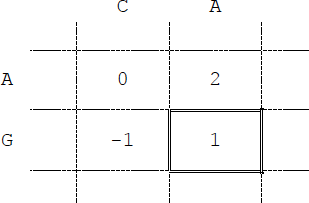
\includegraphics[width=0.25 \textwidth]{fig02/backtrack_recalculate_1.png}
\end{figure}
\begin{solution}[0.25 in]
Vertical
\end{solution}

\item Table 2
\begin{figure}[h]
  \centering
      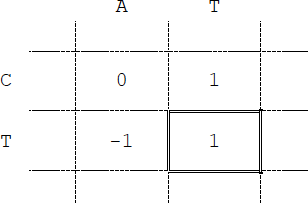
\includegraphics[width=0.25 \textwidth]{fig02/backtrack_recalculate_2.png}
\end{figure}
\begin{solution}[0.25 in]
Diagonal
\end{solution}

\end{itemize}

%% (b)
\part Use backtracking to find the optimal global alignment.
\begin{figure}[h]
  \centering
      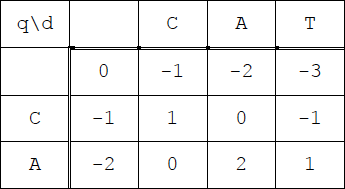
\includegraphics[width=0.3 \textwidth]{fig02/backtrack_simple_table.png}
\end{figure}
\begin{solution}[0.75 in]
\begin{verbatim}
  q: CA-
  d: CAT
\end{verbatim}
\end{solution}

\end{parts}

\bigskip 
